\chapter{Modelo de Datos}
\label{modelo_datos}

La capa de persistencia en el SITEM esta soportada en una estructura de base de datos de modelo Relacional. La forma normal básica - 3NF, se garantiza mientras que otras formas normales pueden ser omitidas en casos puntuales donde se demuestre, por pruebas de desempeño, que no seguirlas redunda en una mejora significativa de la velocidad en el acceso a los datos sin detrimento de la calidad e integridad de los mismos. A continuación se listan las formas normales tenidas en cuenta como patrón de diseño en el modelo de datos del SITEM:

\begin{itemize}
\item Primera Forma Normal: Cada renglón-columna contiene valores atómicos.
\item Segunda Forma Normal: 1NF y todo campo que no sea clave primaria depende de los campos clave.
\item Tercera Forma Normal: 2NF y no hay dependencias transitivas.
\item Forma Normal de Boyce-Codd: Todos los determinantes de la tabla son clave candidata.
\item Cuarta Forma Normal:  Una fila no debe contener dos o más campos multi-valorados.
\item Quinta Forma Normal: Una tabla puede almacenar atributos dependientes a la clave sólo por unión.
\end{itemize}

\begin{figure}
 \centering
 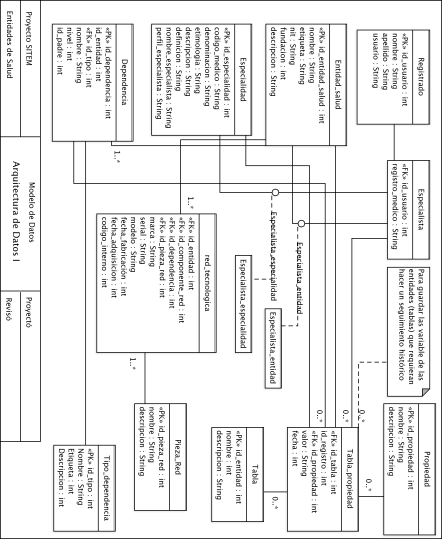
\includegraphics[width=156mm, height=182mm]{datos_entidad.png}
 \caption{Arquitectura de datos Subsistema Entidades de Salud}
 \label{mapanavegacion}
\end{figure}